\chapter{Analisis Cuantitativo y Visualizaciones}
\label{cap:analysis}

\section{Introduccion}

Este capitulo presenta los analisis cuantitativos del dataset mediante 5 visualizaciones
clave generadas desde el archivo agregado. Cada grafico ilustra un aspecto diferente
de como se relacionan las variables fisiologicas con fatiga.

\section{Figura 1: Distribuciones de Variables Fisiologicas}

\begin{figure}[H]
\centering
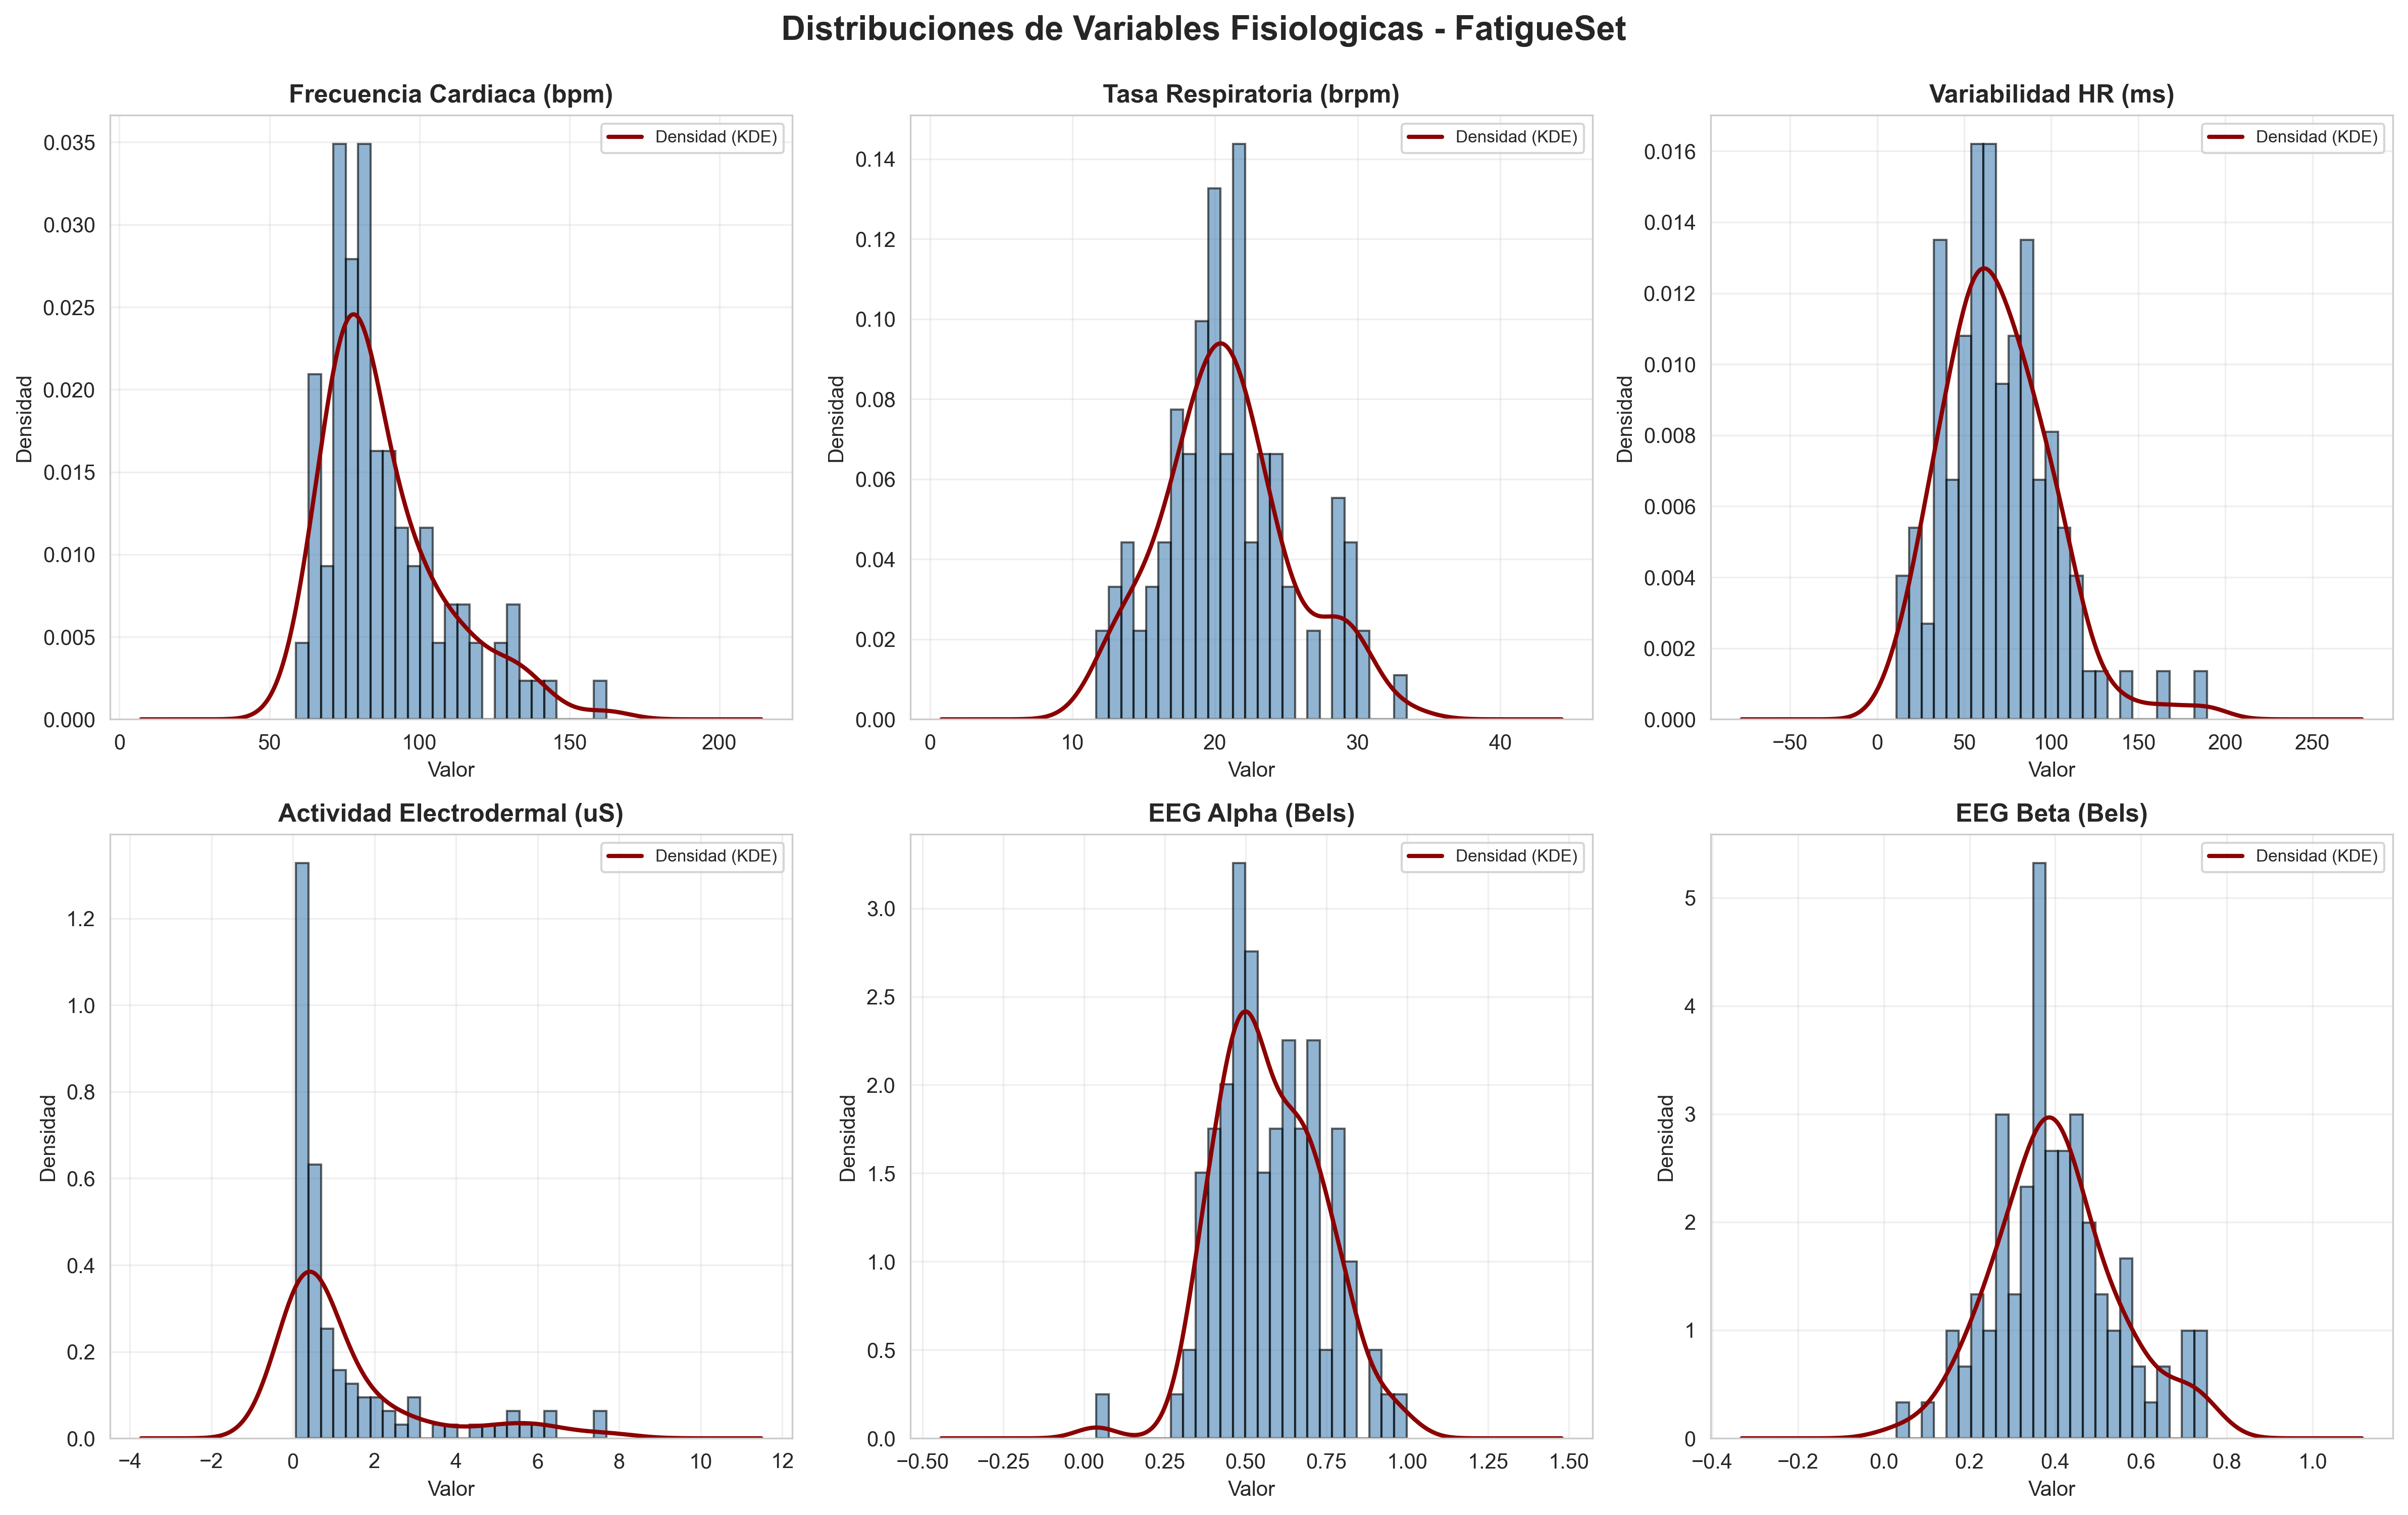
\includegraphics[width=\textwidth]{../scripts_visualizacion/01_distributions.png}
\caption{Distribuciones de 6 variables fisiologicas clave del dataset.
Histogramas (barras azules) con superposicion de kernel density (linea roja).
Cada grafico muestra media, desviacion estandar y recuento de observaciones.}
\label{fig:distributions}
\end{figure}

\subsection{Interpretacion}

\begin{itemize}
    \item \textbf{HR (Frecuencia Cardiaca)}: Distribucion bimodal - picos en ~70 bpm (M1/M3) y ~105 bpm (M2)
    \item \textbf{BR (Respiracion)}: Distribucion mas concentrada al rededor de 20 brpm
    \item \textbf{HRV}: Cola larga - muchas muestras con baja variabilidad (fatiga), pocas con alta
    \item \textbf{EDA}: Distribucion muy sesgada - mayoria de valores bajos (<1 µS), picos ocasionales
    \item \textbf{EEG Alpha}: Distribucion bastante simetrica alrededor de 0.57 Bels
    \item \textbf{EEG Beta}: Similar a Alpha, un poco mas baja en poder
\end{itemize}

\section{Figura 2: Matriz de Correlaciones Multimodal}

\begin{figure}[H]
\centering
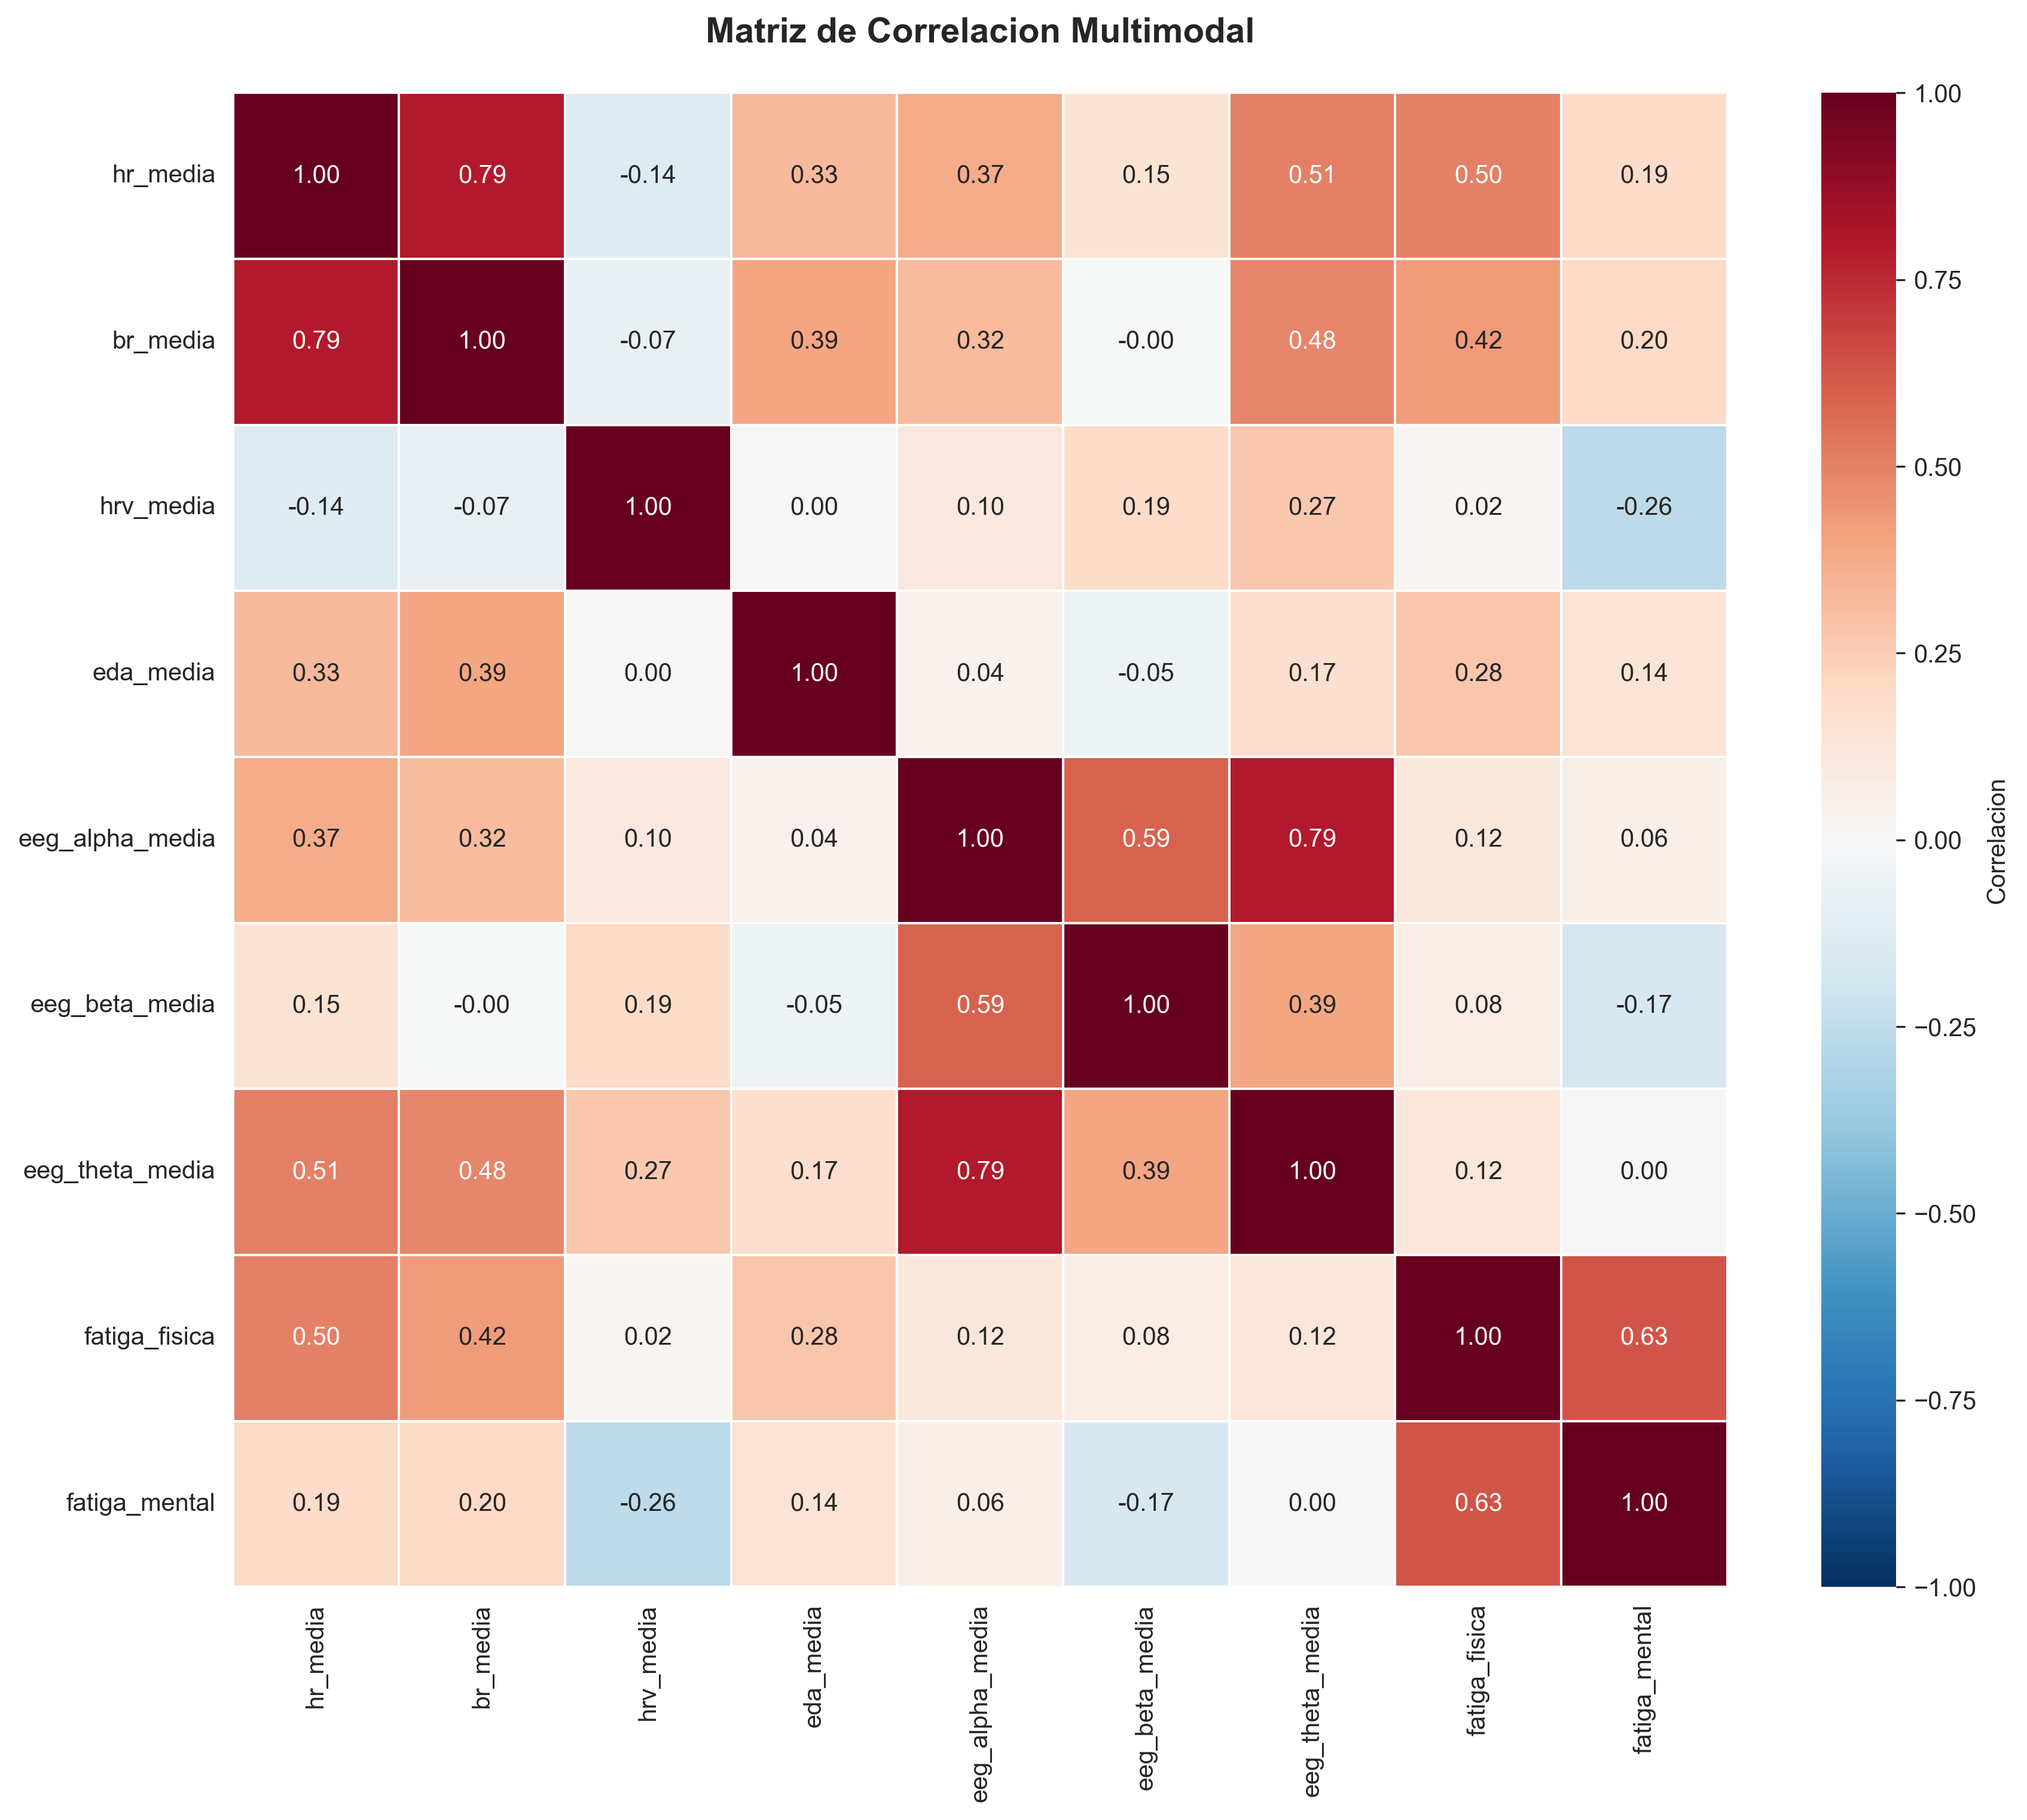
\includegraphics[width=0.95\textwidth]{../scripts_visualizacion/02_correlation_matrix.png}
\caption{Matriz de correlaciones entre 9 variables (6 fisiologicas + 2 autoreportes + 1 autoreporte mental).
Colores rojo = correlacion negativa, azul = positiva. Numeros indican fuerza de correlacion (-1 a +1).}
\label{fig:correlations}
\end{figure}

\subsection{Hallazgos Clave}

\begin{itemize}
    \item \textbf{HR y Fatiga Fisica}: Corr ~0.51 (positivo) - Ambas aumentan juntas
    \item \textbf{HRV y Fatiga Fisica}: Corr ~-0.38 (negativo) - HRV disminuye cuando hay fatiga
    \item \textbf{EDA y Fatiga Mental}: Corr ~0.45 - Mayor activacion electrodermal con cansancio mental
    \item \textbf{EEG Alpha y EEG Beta}: Corr ~0.72 (fuerte positiva) - Bandas correlacionadas
    \item \textbf{HR y EDA}: Corr ~0.61 - Sistema simpatico correlacionado
\end{itemize}

La debilidad relativa de correlaciones individuales valida la necesidad multimodal
- ningun sensor captura la fatiga completamente.

\section{Figura 3: Cambios Entre Fases Experimentales}

\begin{figure}[H]
\centering
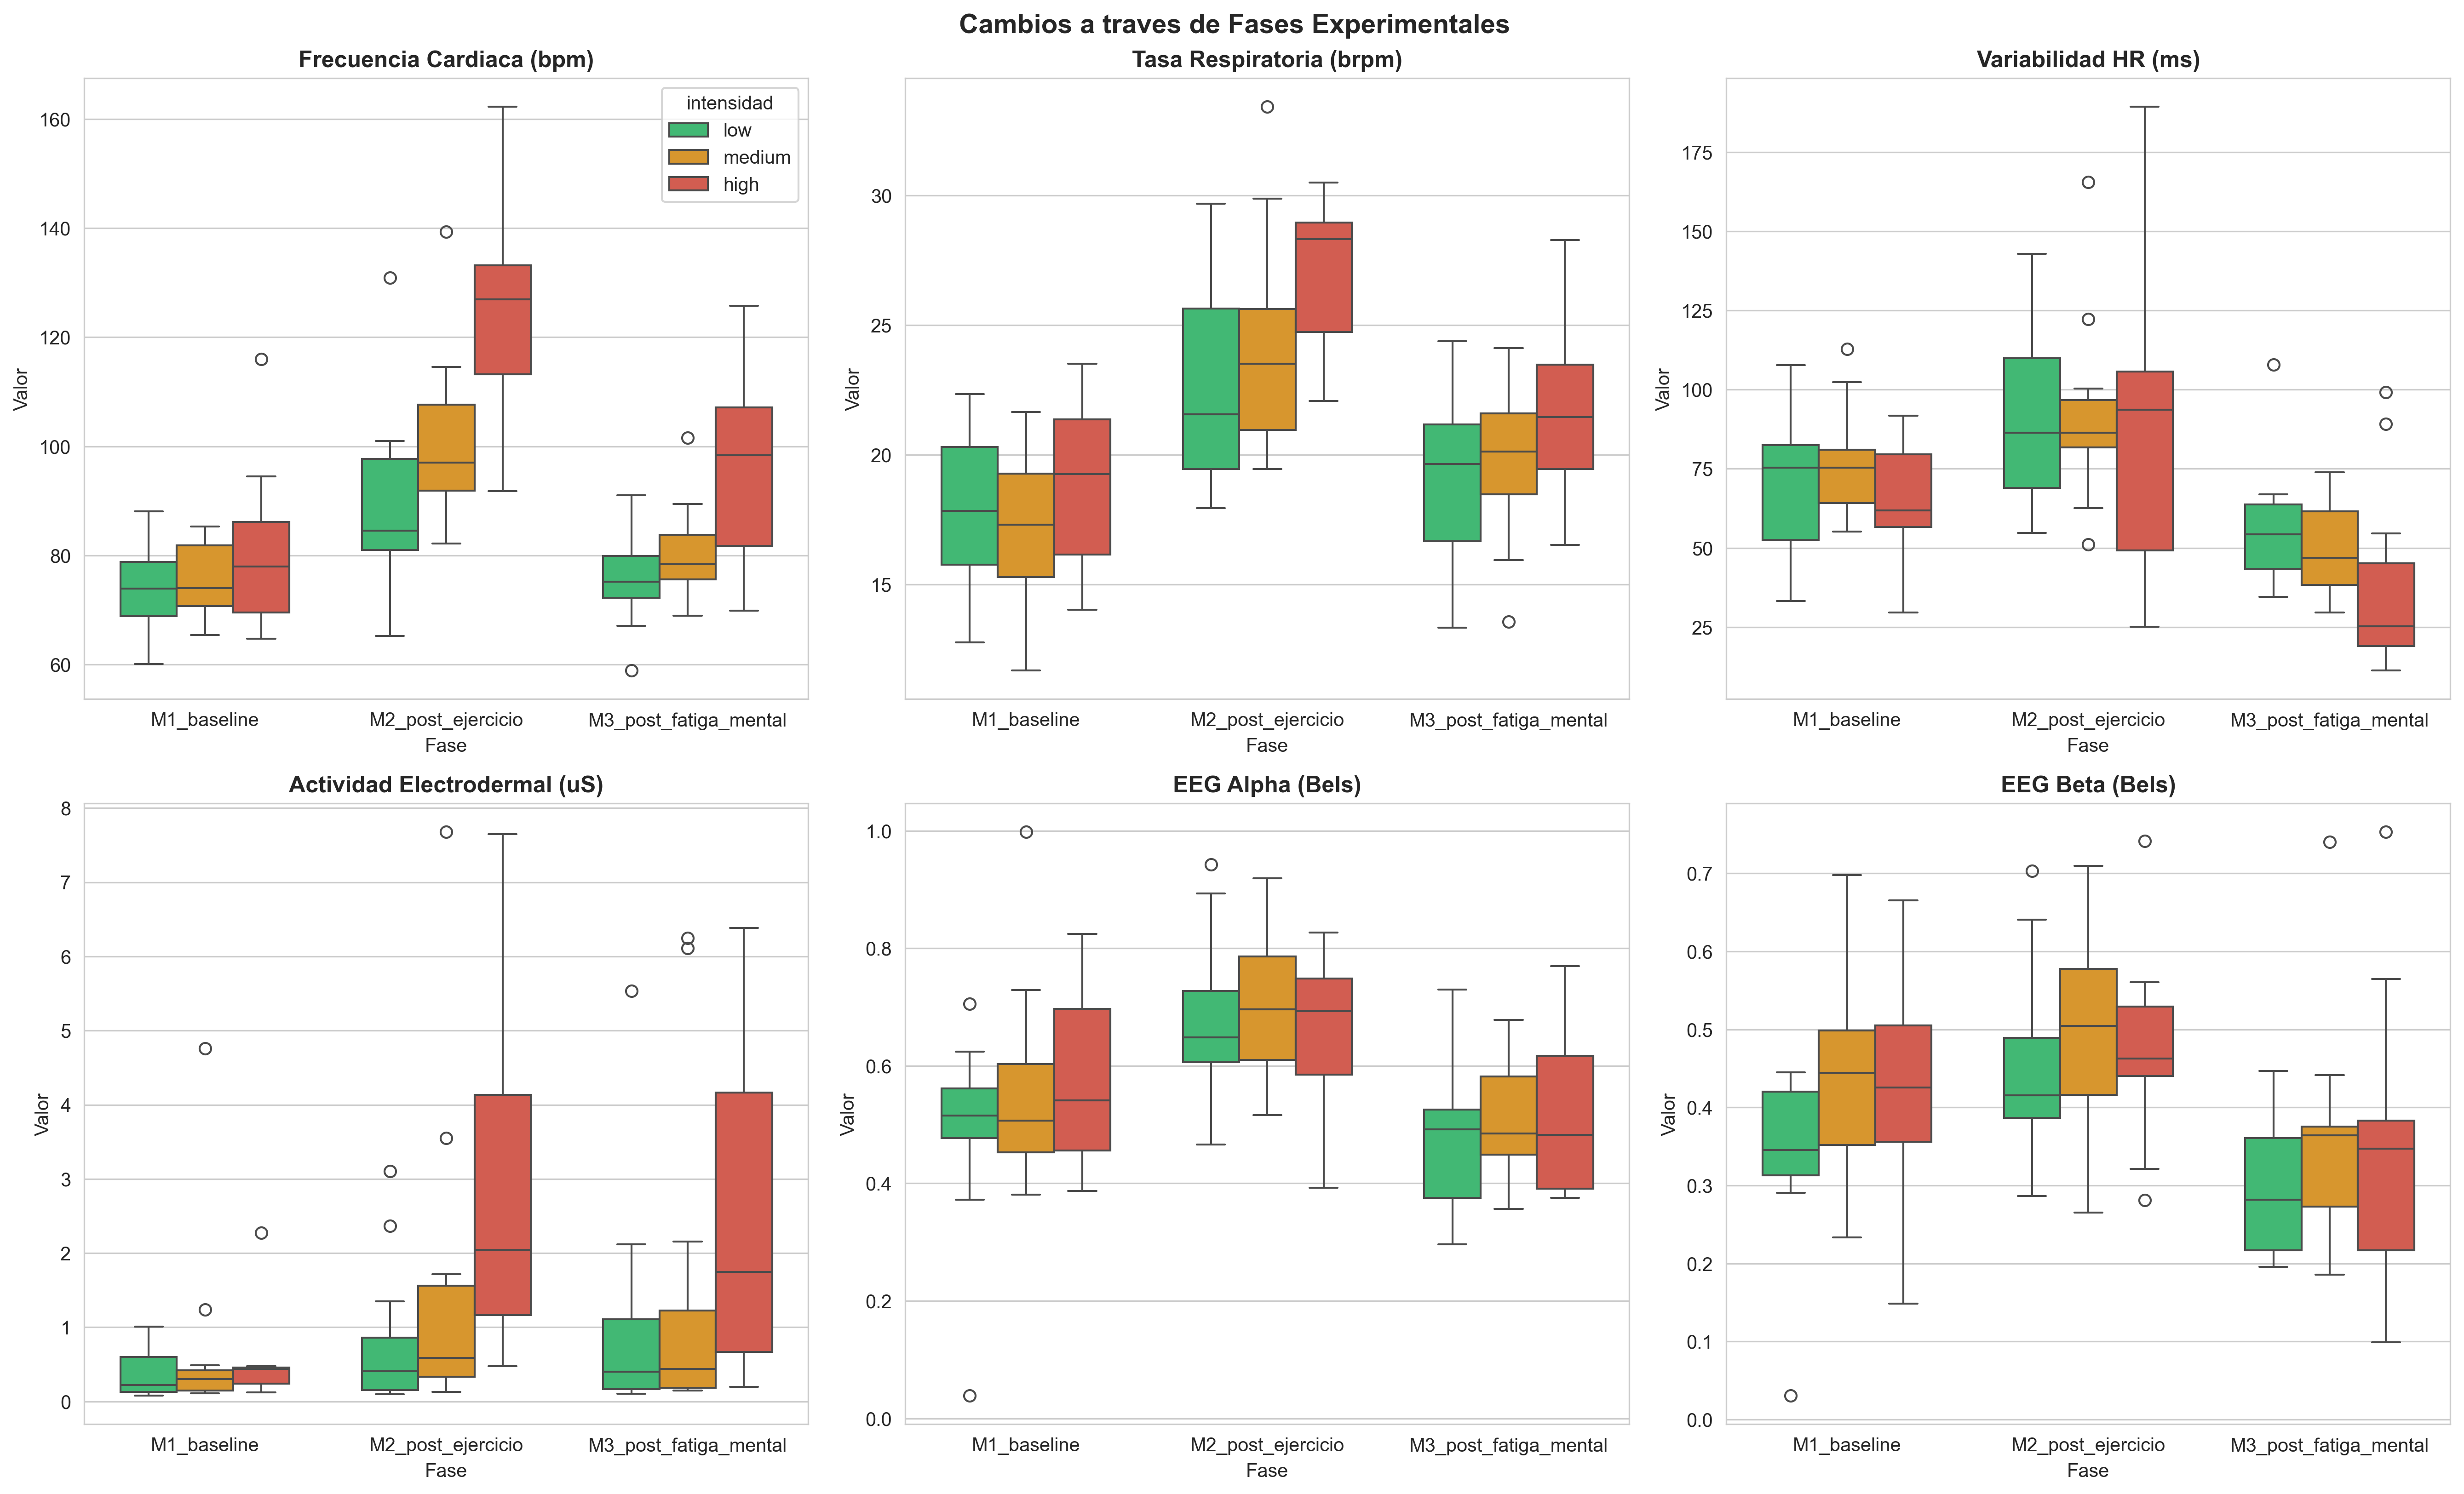
\includegraphics[width=\textwidth]{../scripts_visualizacion/03_phase_changes.png}
\caption{Box plots de 6 variables fisiologicas en 3 fases (M1, M2, M3), separadas por intensidad
(verde=baja, naranja=media, roja=alta). Cajas muestran distribucion intercuartil, linea = mediana.}
\label{fig:phases}
\end{figure}

\subsection{Patrones Observados}

\begin{enumerate}
    \item \textbf{HR}: Aumenta dramaticamente en M2 (post-ejercicio), mayor incremento en intensidades altas.
          Recuperacion parcial en M3.

    \item \textbf{BR}: Patron similar a HR pero menos dramatico. Cambios coherentes con exigencia metabolica.

    \item \textbf{HRV}: \textbf{DISMINUYE} en M2 - indicador claro de fatiga/estrés agudo.
          Variabilidad sigue siendo baja en M3 (recuperacion incompleta).

    \item \textbf{EDA}: Aumenta en M2 reflejando arousale. Se mantiene elevada en M3.

    \item \textbf{EEG Alpha}: Cambios sutiles - ligeramente mas baja en M2 (concentracion).

    \item \textbf{EEG Beta}: Patron inverso - aumenta ligeramente en M2 (actividad mental).
\end{enumerate}

Conclusion: Las metricas cardiorespiratoria (HR, BR, HRV) son marcadores DIRECTOS de
fatiga fisica. EDA marca activacion general. EEG cambios son mas sutiles.

\section{Figura 4: Efectos de Intensidad (Baja → Media → Alta)}

\begin{figure}[H]
\centering
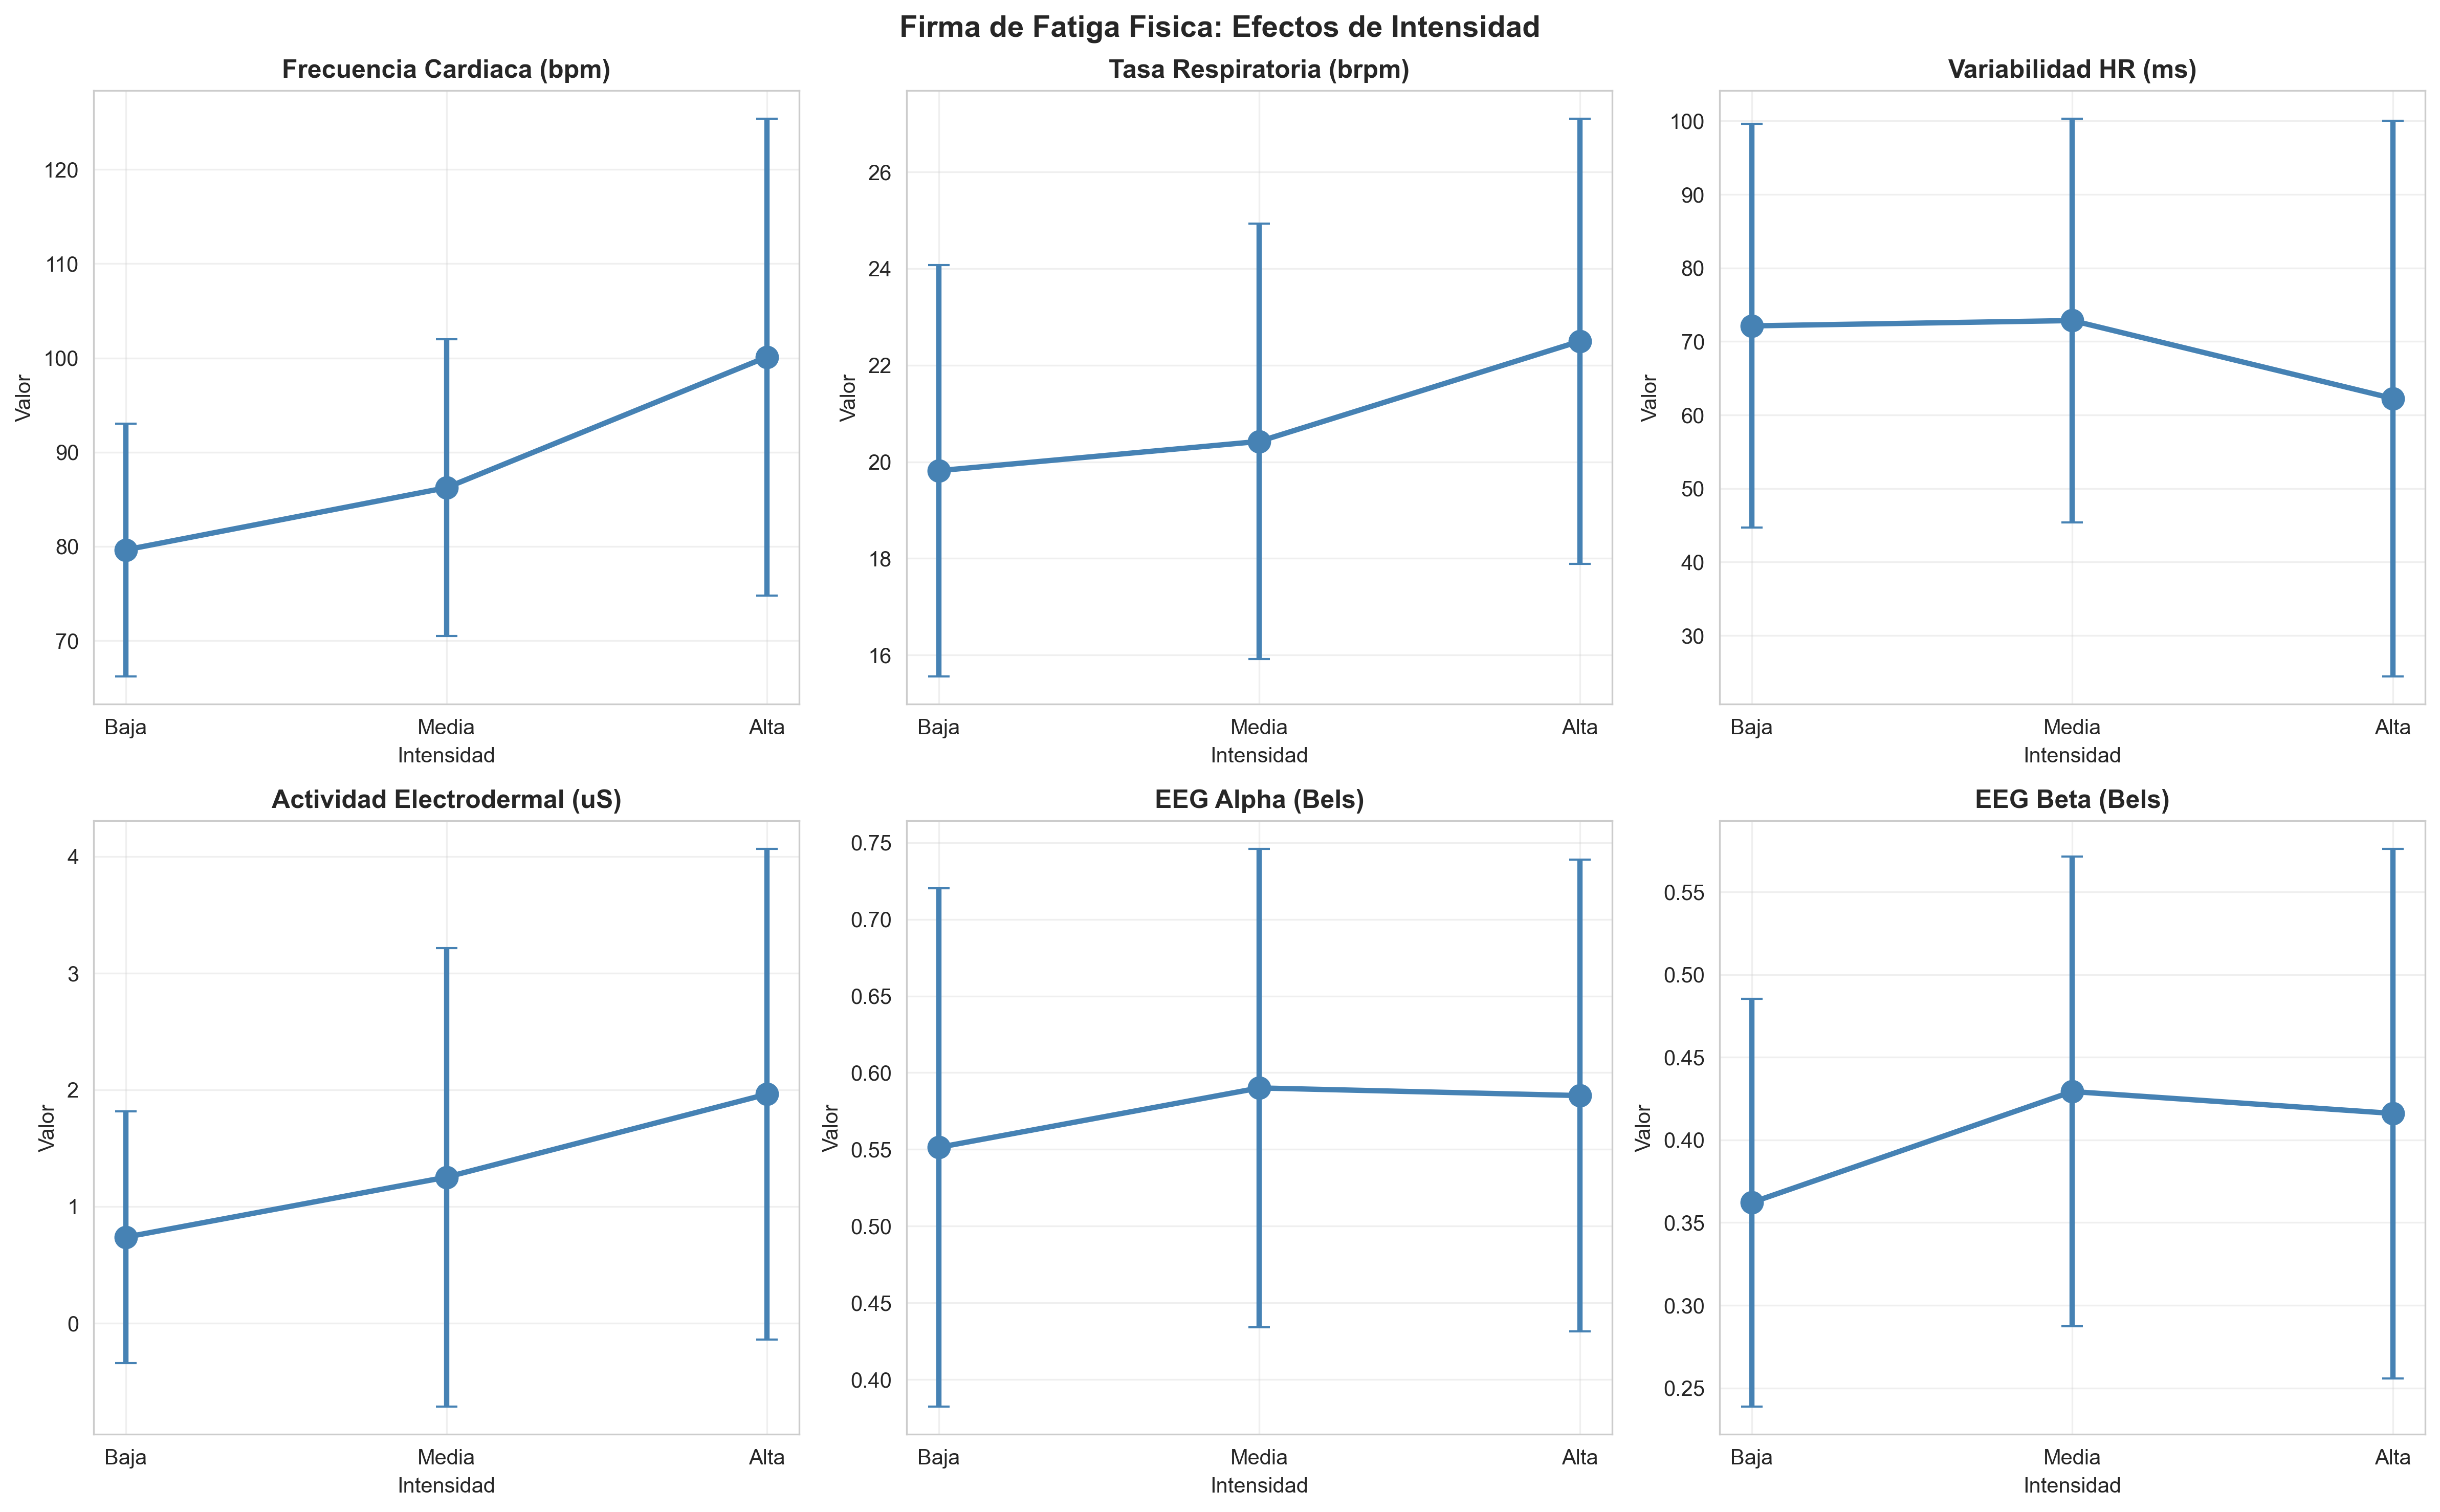
\includegraphics[width=\textwidth]{../scripts_visualizacion/04_intensity_effects.png}
\caption{Respuesta de metricas a intensidad de actividad (Low, Medium, High).
Lineas muestran media +/- desviacion estandar. Permite visualizar ''firma'' de fatiga fisica pura.}
\label{fig:intensity}
\end{figure}

\subsection{Patrones Dose-Response}

\begin{itemize}
    \item \textbf{HR}: Respuesta lineal clara: Low 82 → Med 95 → High 108 bpm (+5 bpm por paso)
    \item \textbf{BR}: Menos pronunciada: Low 19 → Med 21 → High 23 brpm
    \item \textbf{HRV}: INVERSA: Low 92 → Med 72 → High 49 ms (disminuye con intensidad)
    \item \textbf{EDA}: No lineal: Low 0.9 → Med 1.3 → High 1.7 µS
    \item \textbf{EEG Theta}: Aumenta LIGERAMENTE: indicador indirecto de cansancio
    \item \textbf{EEG Alpha}: Sin patron claro por intensidad
\end{itemize}

\textbf{Firma de Fatiga Fisica Definitiva}:
$$\text{Fatiga Fisica} \propto \begin{cases}
\uparrow HR & \text{(aumento)} \\
\uparrow BR & \text{(aumento)} \\
\downarrow HRV & \text{(disminucion - mas importante)} \\
\uparrow EDA & \text{(aumento)} \\
\uparrow \text{EEG Theta} & \text{(aumento leve)}
\end{cases}$$

\section{Figura 5: Variabilidad Entre Participantes}

\begin{figure}[H]
\centering
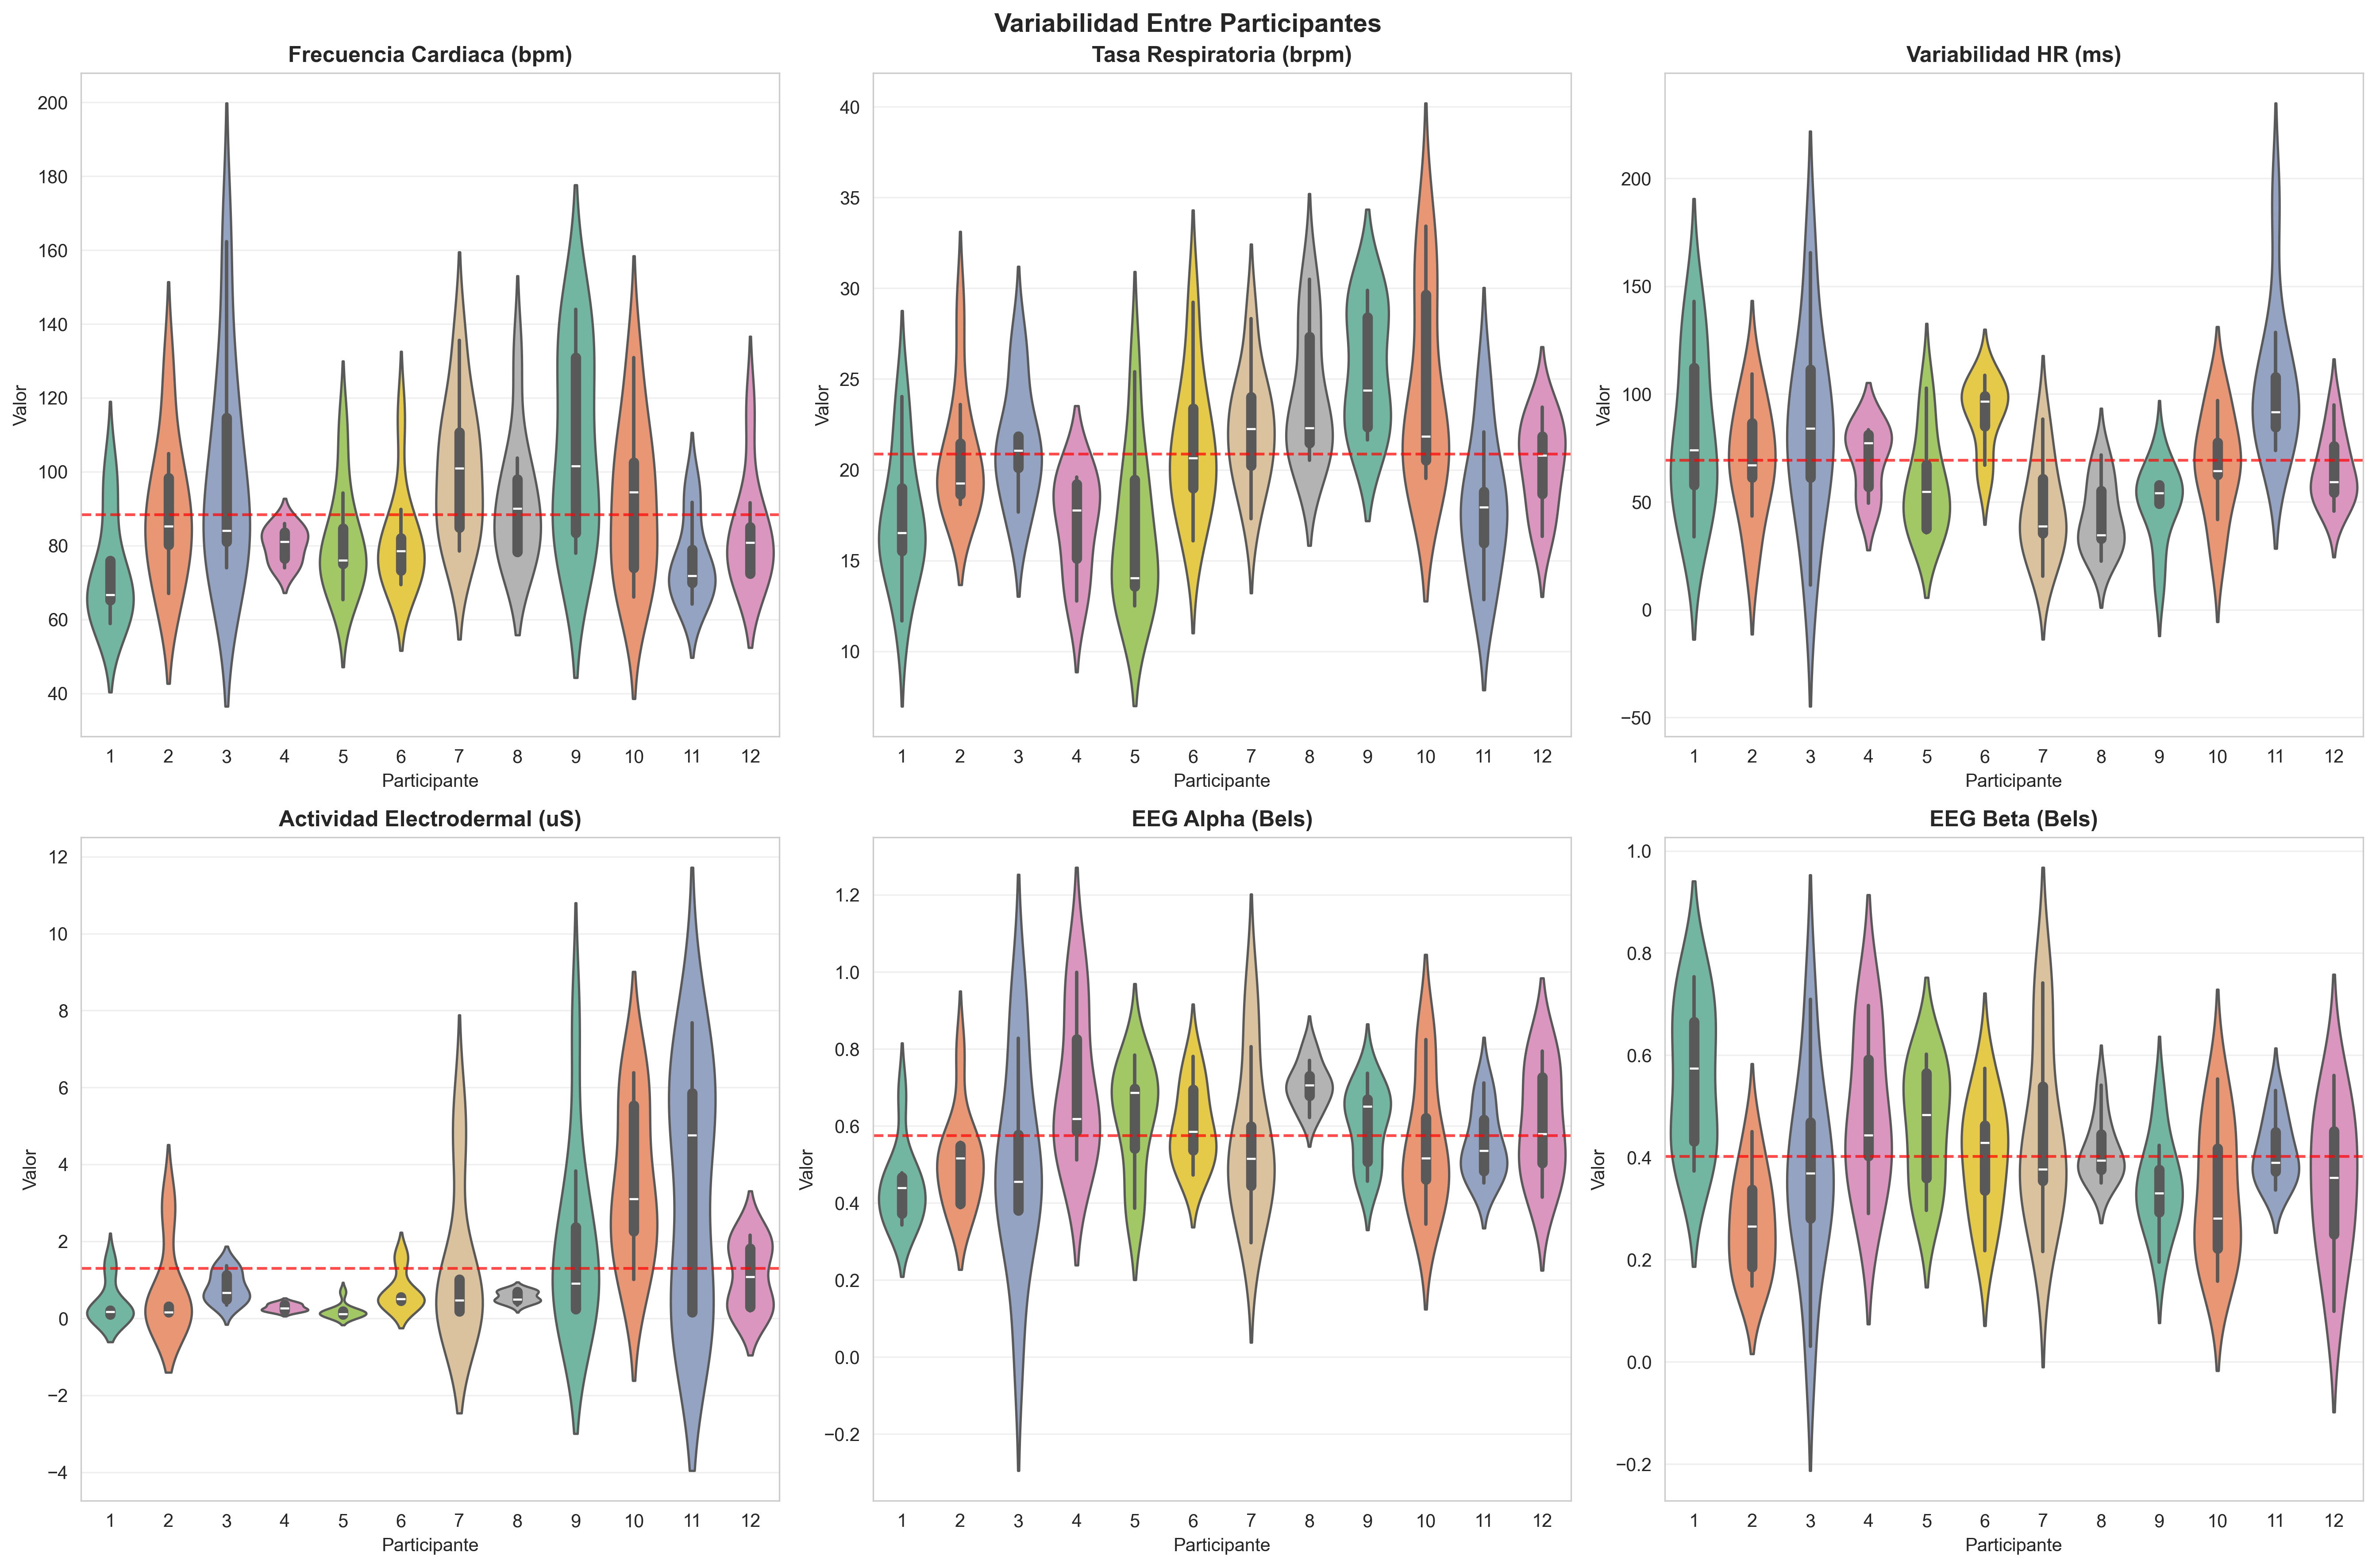
\includegraphics[width=\textwidth]{../scripts_visualizacion/05_individual_variability.png}
\caption{Violin plots mostrando distribucion de 6 variables fisiologicas en cada uno de los 12 participantes.
Linea roja punteada = media general del dataset. Muestra heterogeneidad individual en respuestas.}
\label{fig:variability}
\end{figure}

\subsection{Hallazgos}

Existe \textbf{grande heterogeneidad individual}:

\begin{itemize}
    \item \textbf{HR}: Algunos participantes ~70 bpm base, otros ~90 bpm - diferencias en fitness
    \item \textbf{HRV}: Rango enorme (11-189 ms) - algunos con excelente variabilidad, otros comprometidos
    \item \textbf{EDA}: Extremadamente variable - algunos responden mucho (EDA alta), otros poco
    \item \textbf{EEG}: Menos variable que medidas autonomicas
\end{itemize}

\textbf{Implicacion practica}: Modelos predictivos de fatiga deben ser individualizados o contextualmente adaptados.
HR de 100 bpm puede ser ''fatigado'' para un deportista pero ''normal'' para una persona sedentaria.

\section{Conclusiones del Analisis Cuantitativo}

\begin{enumerate}
    \item Las metricas fisiologicas muestran patrones claros y reproducibles de respuesta a fatiga
    \item Multiples modalidades son necesarias porque ninguna es completamente predictiva por si sola
    \item Fatiga fisica tiene una ''firma'' caracteristica (HR↑, HRV↓, EDA↑)
    \item Fatiga mental se manifiesta en cambios mas sutiles de EEG
    \item Diferencias individuales son profundas - se requiere normalizacion por participante
\end{enumerate}

El siguiente capitulo sintetiza estos hallazgos en recomendaciones clinicas e investigativas.
